\documentclass[10pt,A4paper,tikz,border=20pt]{standalone}
\usepackage[utf8]{inputenc}
\usepackage[T1]{fontenc}
\usepackage{amsmath}
%\usepackage{amsfonts}
\usepackage{amssymb}
\usepackage{mathtools}
\DeclarePairedDelimiter\abs{\lvert}{\rvert}
\usepackage{tikz}
\usetikzlibrary{shapes,arrows,shapes.misc,shapes.symbols}
\usetikzlibrary{positioning}
\usepackage{gitinfo2}
\usepackage{graphicx}
\renewcommand{\gitMark}{Branch:\,\gitBranch\,@\,\gitAbbrevHash{}; Author:\,\gitAuthorName; Date:\,\gitAuthorIsoDate~\textbullet{}}
\makeatletter
\AddToShipoutPictureBG{%
	\AtPageLowerLeft{%
		\kern2.6cm
		\raisebox{\dimexpr.5\paperheight-.8\height}
		{\rotatebox{90}{\gitMarkFormat\gitMarkPref{} \textbullet{} \gitMark}}%
	}%
}%
\makeatother
\newcommand{\segnomodulo}{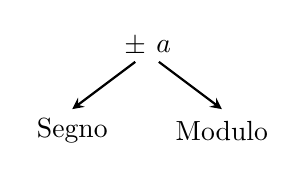
\begin{tikzpicture}[thick]
		\def\x{2.8mm}
		\def\h{8.0mm}
		\def\dist{3mm}%1cm
		\node at (0,0) {$\displaystyle \pm$};
		\node at (1.2*\dist,0) {$a$};
		\node at (-\h,-\h-\x) {Segno};
	\node at (\dist+\h,-\h-\x) {Modulo};
		% collegamento termini
		\draw[-stealth] (0, -0.2)--(0-\h,-\h); 
		\draw[-stealth] (\dist, -0.2)--(\dist+\h,-\h); 
	\end{tikzpicture}%
}
%\renewcommand{\gitMarkFormat}{\color{blue}\sffamily\bfseries}
\begin{document}
\tikzset{
	decision/.style={diamond, draw, %fill=blue!20,
		text width=4.5em, text badly centered, 
		node distance=2.5cm, inner sep=0pt
	},
	block/.style={rectangle, draw, %fill=blue!20,
		text width=15em, 
		text centered, 
		node distance=1.5cm,
		%rounded corners, 
		%minimum height=3em
	},
	loop/.style={chamfered rectangle,chamfered rectangle 	xsep=2cm, draw, %fill=blue!20,
		text width=15em, text centered,  
		node distance=2.5cm,% minimum height=3em
	},
	cloud/.style={draw, ellipse,%fill=red!20, 
		node distance=1.5cm, minimum height=2em
	},
	input/.style={ % requires library shapes.geometric
		draw,
		node distance=1.5cm,
		trapezium,
		trapezium left angle=60,
		trapezium right angle=120,
	},
	line/.style={draw, very thick, %color=black!50,
		-latex'},
		print/.style={ % requires library shapes.symbols
		draw,
		tape,
		tape bend top=none
	},
connessione/.style={
draw,
circle,
radius=5pt,
}
}
%	\begin{center}

		\begin{tikzpicture}[scale=1, %node distance = 2.5cm,
			 auto]
			% Place nodes
			\node (titolo) {\segnomodulo};
			\node [cloud,below of=titolo] (init) {Inizio  somma};
			\node [input, below of=init] (passo1) {Leggo il primo numero};
		\node[input, below of=passo1] (passo2) {Leggo il secondo numero};
		\node[decision,below of=passo2] (decisione1) {I numeri hanno lo stesso segno?};
\node[block,right of=decisione1, node distance=6cm] (scelta1) {La somma ha lo stesso segno e per modulo la somma dei moduli};
\node[block,below of=decisione1,node distance=3cm] (scelta2) {Determino quale numero ha modulo maggiore};
\node[block,below of=scelta2,node distance=3cm] (scelta3) {La somma ha il segno del numero che ha il modulo maggiore. Il modulo della somma è la differenza tra i moduli. };
\node[connessione, below of=scelta3, node distance=2cm] (nodo1) {};
\node[cloud,below of=nodo1] (fine) {Fine somma};
			\path [line] (init) -- (passo1);
			\path [line] (passo1) -- (passo2);
     		\path [line] (passo2) --  (decisione1);
     		\path [line] (decisione1)--node [near start] {Si}(scelta1);
			\path [line] (decisione1)--node [near start] {No}(scelta2);
			\path [line] (scelta2) --  (scelta3);
			\path[line](scelta3)--(nodo1);
			\path [line] (nodo1) --  (fine);
			\path[line] (scelta1)|-(nodo1);
		\end{tikzpicture}
%	\end{center}
\end{document}